\documentclass[lang=cn,newtx,11pt,scheme=chinese,usesamecnt]{elegantbook}

\title{计算方法作业答案}

\author{陈文轩}
\institute{KFRC}
\date{\today}
\version{1.0.0.1145}


\setcounter{tocdepth}{3}

\logo{logo.jpg}
\cover{cover.png}

% 本文档命令
\usepackage{array}
\newcommand{\ccr}[1]{\makecell{{\color{#1}\rule{1cm}{1cm}}}}
\linespread{1.4}

% 修改标题页的橙色带
\definecolor{customcolor}{HTML}{1F1E33}
\colorlet{coverlinecolor}{customcolor}


\usepackage{cprotect}
\usepackage{xcolor}
\usepackage{biblatex}
\usepackage{listings}
\usepackage{graphicx}
\usepackage{amsmath}
\usepackage{mathdots}
\usepackage{extarrows}
\usepackage{tikz}
\usepackage{rotating}
\usepackage{color}
\usepackage{amssymb}
\usepackage{float}
\usepackage{mathtools}
\usepackage{textcomp}
\usepackage{pgfplots}
\pgfplotsset{compat=1.18}



\allowdisplaybreaks[4]


\elegantnewtheorem{homework}{作业}{prostyle}{exfancy}

\everymath{\displaystyle}

\newcommand*{\diff}{\mathop{}\!\mathrm{d}}

\DeclareMathOperator*{\st}{s.t.\,\,}
\DeclareMathOperator*{\argmin}{arg\,min}

\addbibresource[location=local]{reference2.bib} % 参考文献,不要删除

\begin{document}

\maketitle
\frontmatter

\tableofcontents

\mainmatter

\chapter{第一次作业}

    \begin{homework}[10pts]
        对$a>0,n\in\mathbb{N_+}$,$x$很靠近$0$,给出$f(x)$的可靠数值计算方法,使其尽量达到更好的精度:$f(x)=(a+x)^n-a^n$。
    \end{homework}

    \begin{solution}
        $f(x)=(a+x)^n-a^n=\sum\limits_{k=1}^n C_n^k x^k a^{n-k}=(\cdots((x+C_n^1 a)x+C_n^2 a^2)x\cdots+C_n^{n-1}a^{n-1})x$
    \end{solution}

    \begin{homework}[4pts]
        对$a>0$,$x$很靠近$0$,给出$f(x)$的可靠数值计算方法,使其尽量达到更好的精度:$f(x)=\cos(a-x)-\cos a$。
    \end{homework}

    \begin{solution}
        \begin{flalign*}
            f(x)&=\cos(a-x)-\cos a=\cos a\cos x+\sin a\sin x-\cos a &\\
                &=\cos a(\cos x-1)+\sin a\sin x\approx-\frac{1}{2}x^2 \cos a+x\sin a &
        \end{flalign*}
    \end{solution}

    \begin{homework}[4pts]
        对$x\gg a$,给出$f(x)$的可靠数值计算方法,使其尽量达到更好的精度:$f(x)=\sqrt{x^2+a}-x$。
    \end{homework}

    \begin{solution}
        $f(x)=\sqrt{x^2+a}-x=\dfrac{x^2+a-x^2}{\sqrt{x^2+a}+x}=\dfrac{a}{\sqrt{x^2+a}+x}$
    \end{solution}

    \begin{homework}[4pts]
        设有精确值$x^{*}=2023.0905$,则其近似值$x_1=2023.090,x_2=2023.0900$分别有几位有效数字?
    \end{homework}

    \begin{solution}
        $x_1$有$7$位有效数字,$x_2$有$7$位有效数字。
    \end{solution}





\chapter{第二次作业}

    \begin{homework}[6pts]
        (利用下面的函数值表,作差商表,写出相应的牛顿插值多项式以及插值误差表达式,并计算$f(1.5)$和$f(4)$的近似值:
            \begin{table}[H]
                \begin{center}
                    \begin{tabular}{|c|c|c|c|c|}
                    \hline
                    $x$ & $1.0$ & $2.0$ & $3.0$ & $4.5$ \\
                    \hline
                    $f(x)$ & $2.5$ & $4.0$ & $3.5$ & $2.0$ \\
                    \hline
                    \end{tabular}
                \end{center}
            \end{table}
    \end{homework}

    \begin{solution}
        先计算各阶差商:$f[x_0]=2.5,f[x_1]=4,f[x_2]=3.5,f[x_3]=2;$
        
        $f[x_0,x_1]=\frac{f[x_1]-f[x_0]}{x_1-x_0}=1.5,f[x_1,x_2]=\frac{f[x_2]-f[x_1]}{x_2-x_1}=-0.5,f[x_2,x_3]=\frac{f[x_3]-f[x_2]}{x_3-x_2}=-1;$

        $f[x_0,x_1,x_2]=\dfrac{f[x_1,x_2]-f[x_0,x_1]}{x_2-x_0}=-1,f[x_1,x_2,x_3]=\dfrac{f[x_2,x_3]-f[x_1,x_2]}{x_3-x_1}=-0.2;$

        $f[x_0,x_1,x_2,x_3]=\dfrac{f[x_0,x_1,x_2]-f[x_1,x_2,x_3]}{x_3-x_0}=\dfrac{8}{35}.$

        因此,插值多项式$P_3(x)=2.5+1.5(x-1)-(x-1)(x-2)+\dfrac{8}{35}(x-1)(x-2)(x-3),$

        完全展开可以得到$P_3(x)=\dfrac{8}{35}x^3-\dfrac{83}{35}x^2+\dfrac{491}{70}x-\dfrac{83}{35}.$

        误差项$R_3(x)=\dfrac{f^{(4)}(\xi)}{24}(x-1)(x-2)(x-3)(x-4.5),\xi\in[1,4.5].$

        $P_3(1.5)=\dfrac{251}{70},P_3(4)=\dfrac{83}{35}.$
    \end{solution}

    \begin{homework}[6pts]
        利用数据$f(0)=2.0,f(1)=1.5,f(3)=0.25,f'(3)=1$构造出三次插值多项式,写出其插值余项,并计算$f(2)$的近似值。
    \end{homework}

    \begin{solution}
        设插值多项式$P_3(x)=a_{3}x^3+a_2 x^2+a_1 x_1+a_0$,对应$P_3 '(x)=3a_3 x^2+2a_2 x+a_1;$
        
        则有$P_3(0)=a_0=2,P_3(1)=a_3+a_2+a_1+a_0=1.5,P_3 '(3)=27a_3+6a_2+a_1=1$

        $ P_3(3)=27a_3+9a_2+3a_1+a_0=0.25\Rightarrow a_3=\dfrac{41}{144},a_2=-\dfrac{85}{72},a_1=\dfrac{19}{48},a_0=2$

        所以插值函数为$P_3(x)=\dfrac{41}{144}x_3-\dfrac{85}{72}x^2+\dfrac{19}{48}x+2$,

        余项为$R_3(x)=\dfrac{f^{(4)}(\xi)}{24}x(x-1)(x-3)^2,\xi\in[0,3];P_3(2)=\dfrac{25}{72}$
    \end{solution}

    \begin{homework}[6pts]
        设$f(x)=20x^3-x+2024$,求$f[1,2,4]$和$f[1,2,3,4]$;
    \end{homework}

    \begin{solution}
        $f[1]=2043,f[2]=2182,f[3]=2561,f[4]=3300;$
        
        $f[1,2]=139,f[2,3]=379,f[3,4]=739,f[2,4]=559;$

        $f[1,2,3]=120,f[2,3,4]=180,\color{red}{f[1,2,4]=140};$

        $\color{red}{f[1,2,3,4]=20}.$
    \end{solution}

    \begin{homework}[6pts]
        设$\{l_i(x)\}_{i=0}^6$是以$\{x_i=2i\}_{i=0}^6$为节点的$6$次Lagrange插值基函数,求$\sum\limits_{i=0}^6 (x_i^3+x_i^2+1)l_i(x)$和$\sum\limits_{i=0}^6 (x_i^3+x_i^2+1)l_i'(x)$,结果需要化简。
    \end{homework}

    \begin{solution}
        记$f(x)=x^3+x^2+1$,则$l_i(x)$可以看作对$f(x)$插值时的基函数。由于节点数量为7,
        
        $\deg f(x)=3$,所以$\sum\limits_{i=0}^6 (x_i^3+x_i^2+1)l_i(x)=f(x)=x^3+x^2+1,$

        $\sum\limits_{i=0}^6 (x_i^3+x_i^2+1)l_i'(x)=f'(x)=3x^2+2x.$
    \end{solution}

    \begin{homework}[6pts]
        设$x_0,x_1,\cdots,x_n(n>2)$为互异的节点,$l_k(x)(k=0,1,\cdots,n)$为与其对应的$n$次Lagrange插值基函数,证明$\sum\limits_{k=0}^n (x_k-x)^n l_k(x)=0$。
    \end{homework}

    \begin{solution}
        \begin{flalign*}
            \qquad \sum_{k=0}^n (x_k-x)^n l_k(x) &= \sum_{k=0}^n \sum_{m=0}^n \left(\binom{n}{m}x_k^{n-m}(-x)^m\right) l_k(x)  & \\
                &= \sum_{m=0}^n \binom{n}{m} (-x)^m \sum_{k=0}^n x_k^{n-m} l_k(x) =\sum_{m=0}^n \binom{n}{m}(-x)^m x^{n-m} & \\
                &=(x-x)^n\equiv 0 & \\
        \end{flalign*}
    \end{solution}

\chapter{第三次作业}

    \begin{homework}[6pts]
        构造积分$\bar{I}(f)=\int_{-h}^{2h}f(x)\diff x$的数值积分公式$I(f)=a_{-1}f(-h)+a_0 f(0)+a_1 f(2h)$,$h>0$;
    \end{homework}

    \begin{solution}
        积分对$p_0(x)=1,p_1(x)=x,p_2(x)=x^2$无误差,对应方程组$\begin{cases}a_{-1}+a_0+a_1=3h\\-2a_{-1}+4a_1=3h\\a_{-1}+4a_1=3h\end{cases}$

        $\Rightarrow a_{-1}=0,a_0=2.25h,a_1=0.75h,I(f)=\dfrac94 hf(0)+\dfrac34 hf(2h).$
    \end{solution}

    \begin{homework}[6pts]
        分别利用梯形公式和Simpson公式求如下积分及其误差(计算结果至少保留小数点后4位):$\int_0^2 e^{-x}\sin x\diff x$
    \end{homework}

    \begin{solution}
        准确值:$\int_0^2 e^{-x}\sin x\diff x=-\dfrac12 e^{-x}(\sin x+\cos x)\Big|_0^2\approx 0.46663$;

        $ f(0)=0,f(1)\approx0.30956,f(2)\approx0.12306$;

        Simpson公式:$I_1=\dfrac{b-a}6\left(f(a)+4f\left(\dfrac{a+b}2\right)+f(b)\right)\approx0.4538$,误差约为$0.0128$;

        梯形公式:$I_2=\dfrac{b-a}{2}(f(a)+f(b))\approx0.12306$,误差约为$0.3436$。
    \end{solution}

    \begin{homework}[10pts]
        记$I(f)=\int_{-2}^2 f(x)\diff x$,设$S(f(x))$为其数值积分公式,其中$I(f)\approx S(f(x))=Af(-\alpha)+Bf(0)+Cf(\alpha)$.
        \begin{enumerate}
            \item 试确定参数$A,B,C,\alpha$使得该数值积分公式具有尽可能高的代数精度,并确定该公式的代数精度(需给出求解过程);
            \item 设$f(x)$足够光滑(可微),求该数值积分公式的误差
        \end{enumerate}
    \end{homework}

    \begin{solution}
        取$A=C$,积分对$x^{2k+1}$无误差。积分对$p_0(x)=1,p_2(x)=x^2,p_4(x)=x^4$无误差,

        对应方程组$\begin{cases}2A+B=4\\A\alpha^2=\dfrac83\\A\alpha^4=\dfrac{32}5\end{cases}\Longrightarrow\begin{cases}A=C=\dfrac{10}9\\B=\dfrac{16}9\\\alpha=\dfrac25\sqrt{15}\end{cases}$,代数精度为$5$次。

        误差为$E(f)=\dfrac{E(x^6)}{6!}f^{(6)}(\xi)=\left(\int_{-2}^2 x^6\diff x-S(x^6)\right)\dfrac{f^{(6)}(\xi)}{216}=\dfrac{64}{7875} f^{(6)}(\xi),\xi\in[-2,2]$
    \end{solution}

    \begin{homework}[8pts]
        求满足下表数据以及边界条件$S''(-2)=S''(2)=0(n=3)$的三次样条插值函数$S(x)$,并计算$S(0)$的值。注意:$n$为小区间个数。
        \begin{table}[H]
            \begin{center}
                \begin{tabular}{|c|c|c|c|c|}
                \hline
                $x$ & $-2.00$ & $-1.00$ & $1.00$ & $2.00$ \\
                \hline
                $f(x)$ & $-4.00$ & $2.00$ & $2.50$ & $1.50$ \\
                \hline
                \end{tabular}
            \end{center}
        \end{table}
    \end{homework}

    \begin{solution}
        $S_i(x)=a_i+b_i(x-x_i)+c_i(x-x_i)^2+d_i(x-x_i)^3,i=0,1,2$满足$S(x_i)=f(x_i),i=0,1,2,3$

        记$M_i=S''(x_i)$,则$\dfrac{h_{i-1}}{6}M_{i-1}+\dfrac{h_{i-1}+h_i}{3}M_i+\dfrac{h_i}{6}M_{i+1}=\dfrac{f[x_i,x_{i+1}]-f[x_{i-1},x_i]}{h_i},i=1,2$

        $ M_i=0,i=0,3$,其中$h_i=x_{i+1}-x_i$。现在有$12$个方程与$12$个未知数,解方程组得到:

        $ S(x)=\begin{cases}-4+6.25(x+2)^2-0.25(x+2)^3,&x\in[-2,-1]\\2+1.75(x+1)-0.75(x+1)^2+0.09375(x+1)^3,&x\in[-1,1]\\2.5-0.9375(x-1)-0.1875(x-1)^2+0.0625(x-1)^3,&x\in[1,2]\end{cases}$

        故$S(0)=3.5625=\dfrac{57}{16}$

    \end{solution}

\chapter{第四次作业}

    \begin{homework}[6pts]
        给定函数$f(x)$离散值如下:
            \begin{table}[H]
                \begin{center}
                    \begin{tabular}{|c|c|c|c|c|}
                    \hline
                    $x$ & $0.00$ & $0.02$ & $0.04$ & $0.06$ \\
                    \hline
                    $f(x)$ & $2.5$ & $1.0$ & $2.0$ & $3.5$ \\
                    \hline
                    \end{tabular}
                \end{center}
            \end{table}
            分别用向前、向后以及中心差商公式计算$f'(0.02)$和$f'(0.04)$;
    \end{homework}

    \begin{solution}
        向前差分:$f'(0.02)=\dfrac{f(0.04)-f(0.02))}{0.02}=50,f'(0.04)=\dfrac{f(0.06)-f(0.04)}{0.02}=75;$

        向后差分:$f'(0.02)=\dfrac{f(0.02)-f(0.00)}{0.02}=-75,f'(0.04)=\dfrac{f(0.04)-f(0.02)}{0.02}=50;$

        中心差分:$f'(0.02)=\dfrac{f(0.04)-f(0.00)}{0.04}=-12.5,f'(0.04)=\dfrac{f(0.06)-f(0.02)}{0.04}=62.5$。
    \end{solution}

    \begin{homework}[8pts]
        用$3$点的Gauss-Legendre数值积分公式求积分$\int_0^2 e^{-x}\sin(x)\diff x$及其积分误差;
    \end{homework}

    \begin{solution}
        准确值:$0.4666$。先换元$\int_{-1}^1 e^{-t-1}\sin(t+1)\diff t$,记$g(t)=e^{-t-1}\sin(t+1)$,

        $I(g)=\dfrac59 g\left(-\sqrt{\dfrac35}\right)+\dfrac89 g(0)+\dfrac59 g\left(\sqrt{\dfrac35}\right)\approx0.4665$,
    \end{solution}

    \begin{homework}[8pts]
        试推导积分$\int_0^2 (x-1)^2 f(x)\diff x$的$2$点Gauss积分公式,这里$(x-1)^2$为权重函数;
    \end{homework}

    \begin{solution}
        先换元为$\int_{-1}^1 t^2 f(t+1)\diff t$,此时$\alpha_1=-\sqrt{\dfrac35},\alpha_2=\sqrt{\dfrac35}$,由于对称性,权重相等,代入

        $f(t)=1$时无误差,得到$W_1=W_2=\dfrac13$,故$I(f)=\dfrac13 f\left(1-\sqrt{\dfrac35}\right)+\dfrac13f\left(1+\sqrt{\dfrac35}\right)$。
    \end{solution}

    \begin{homework}[10pts]
        设函数$f(x)$充分光滑(可微),试推导如下数值微分公式(即确定常数$A,B,C,D,E$),使其截断误差为$O(h^4),f'(x)=\dfrac1h (Af(x-2h)+Bf(x-h)+Cf(x)+Df(x+h)+Ef(x+2h))$。
    \end{homework}

    \begin{solution}
    作Taylor展开至$O(h^5)$,有:

    $f(x+h)=f(x)+hf'(x)+\dfrac12 h^2 f''(x)+\dfrac16 h^3 f'''(x)+\dfrac1{24} h^4 f''''(x)+O(h^5)$

    $f(x-h)=f(x)-hf'(x)+\dfrac12 h^2 f''(x)-\dfrac16 h^3 f'''(x)+\dfrac1{24} h^4 f''''(x)+O(h^5)$

    $f(x+2h)=f(x)+2hf'(x)+2h^2 f''(x)+\dfrac43 h^3 f'''(x)+\dfrac23 h^4 f''''(x)+O(h^5)$

    $f(x-2h)=f(x)-2hf'(x)+2h^2 f''(x)-\dfrac43 h^3 f'''(x)+\dfrac23 h^4 f''''(x)+O(h^5)$\vspace{-0.9cm}

    \begin{flalign*}
        \qquad\qquad& Af(x-2h)+Bf(x-h)+Cf(x)+Df(x+h)+Ef(x+2h) &\\
        =&(A+B+C+D+E)f(x)+(-2A-B+D+2E)hf'(x)&\\
        &+(2A+\dfrac12 B+\frac12 D+2E)h^2 f''(x)+(-\dfrac 43 A-\dfrac16 B+\dfrac16 D+\dfrac43 E)h^3 f'''(x) &\\
        &+(\dfrac 23 A-\dfrac1{24} B+\dfrac1{24} D+\dfrac23 E)h^4 f''''(x)&\\
        \coloneqq& hf'(x)+O(h^5)&
    \end{flalign*}\vspace{-0.9cm}

    $\Rightarrow\begin{cases}A+B+C+D+E=0\\-2A-B+D+2E=1\\(2A+\dfrac12 B+\frac12 D+2E=0\vspace{0.2cm}\\-\dfrac 43 A-\dfrac16 B+\dfrac16 D+\dfrac43 E=0\vspace{0.2cm}\\\dfrac 23 A-\dfrac1{24} B+\dfrac1{24} D+\dfrac23E=0\end{cases}\Rightarrow\begin{cases}A=\dfrac1{12} \vspace{0.2cm}\\B=-\dfrac23\\ C=0\\D=\dfrac23\vspace{0.2cm}\\E=\dfrac1{12}\end{cases}$

    因此数值微分公式为$f'(x)=\frac{-f(x+2h)+8f(x+h)-8f(x-h)+f(x-2h)}{12h}+O(h^4)$。
    \end{solution}

\chapter{第五次作业}

    \begin{homework}[12pts]
        设有常微分方程初值问题$\begin{cases}y'(x)=-y(x),0\leq x\leq 1\\y(0)=1\end{cases}$,假设求解区间$[0,1]$被$n$等分,令$h=\frac1n,x_k=\frac kn(k=0,1,\cdots,n)$
        \begin{enumerate}
            \item 分别写出用\textcolor{red}{向前Euler公式,向后Euler公式,梯形公式以及改进的Euler公式}求上述微分方程数值解时的差分格式(即\textcolor{blue}{$y_{k+1}$与$y_k$}二者之间的递推关系式);
            \item 设\textcolor{blue}{$y_0=y(0)$},分别求这四种公式(方法)下的近似值\textcolor{blue}{$y_n$}的表达式(注:这里的\textcolor{blue}{$y_n$}即是\textcolor{blue}{$y(x_n)\equiv y(1)$的近似值};
            \item 当\textcolor{blue}{$n$}足够大(即区间长度\textcolor{blue}{$h\rightarrow 0$}时,分别判断四种方法下的近似值\textcolor{blue}{$y_n$}是否收敛到原问题的真解\textcolor{blue}{$y(x)$}在\textcolor{blue}{$x=1$}处的值。
        \end{enumerate}
    \end{homework}

    \begin{solution}
        显然解析解是$y=e^{-x}$,对应$y(1)=e^{-1}$。以下$n=\dfrac1k$。
        \begin{itemize}
            \item 向前Euler公式:$y_{k+1}=y_k+h(-y_k)=(1-h)y_k,y_n=(1-h)^n,\lim\limits_{n\rightarrow \infty}y_n=e^{-1}=y(1)$;
            \item 向后Euler公式:$y_{k+1}=y_k-hy_{k+1}=\dfrac{y_k}{1+h},y_n=\left(\dfrac1{1+h}\right)^n,\lim\limits_{n\rightarrow \infty}y_n=e^{-1}=y(1)$;
            \item 梯形公式:$y_{k+1}=y_k+\dfrac h2(-y_k-y_{k+1})=\dfrac{2-h}{2+h}y_k,y_n=\left(\dfrac{2-h}{2+h}\right)^n\lim\limits_{n\rightarrow \infty}y_n=e^{-1}=y(1)$;
            \item 改进的Euler公式:预测:$y^*=y_k+h(-y_k)=(1-h)y_k$,

                校正:$y_{k+1}=y_k+\dfrac h2(-y_k-y^*)=\left(1-h+\dfrac {h^2} 2\right)y_k,y_n=\left(1-h+\dfrac {h^2} 2\right)^n$,此时$\lim\limits_{n\rightarrow \infty}y_n=e^{-1}=y(1)$。
        \end{itemize}


    \end{solution}

    \begin{homework}[8pts]
        试推导$p=1,q=2$显式公式\textcolor{blue}{$y_{n+1}=y_{n-1}+\dfrac h3\left(7f(x_n,y_n)-2f(x_{n-1},y_{n-1})+f(x_{n-2}\right.$}

        \textcolor{blue}{$\left.,y_{n-2})\right)$}的\textcolor{red}{局部截断误差},即验证\textcolor{blue}{$T_{n+1}\equiv y(x_{n+1})-y_{n+1}=\,\,$}\textcolor{magenta}{$\dfrac13 h^4 y^{(4)}(x_{n-1})+O(h^5)$}

        (提示:\textcolor{magenta}{将差分格式右端点某些项在某点处同时作Taylor展开});
    \end{homework}

    \begin{solution}
        $y(x_{n+1})=y(x_{n-1})+2hy'(x_{n-1})+2h^{2}y''(x_{n-1})+\dfrac43 h^{3}y'''(x_{n-1})+\dfrac23 h^4 y''''(x_{n-1})+O(h^5)$;

        $f(x_n,y_n)=y'(x_n)=y'(x_{n-1})+hy''(x_{n-1})+\dfrac12 h^2 y'''(x_{n-1})+\dfrac16 h^3 y''''(x_{n-1})+O(h^4)$

        $f(x_n,y_{n-2})=y'(x_{n-2})=y'(x_{n-1})-hy''(x_{n-1})+\dfrac12 h^2 y'''(x_{n-1})-\dfrac16 h^3 y''''(x_{n-1})+O(h^4)$

        \begin{flalign*}
            \qquad\quad&y(x_{n+1})-y_{n+1}=y(x_{n+1})-\dfrac h3\left(7f(x_n,y_n)-2f(x_{n-1},y_{n-1})+f(x_{n-2})\right) &\\
            =&y(x_{n-1})+2hy'(x_{n-1})+2h^{2}y''(x_{n-1})+\dfrac43 h^{3}y'''(x_{n-1})+\dfrac23 h^4 y''''(x_{n-1})+O(h^5)-\dfrac h3 &\\
             &\left(7\left(y'(x_{n-1})+hy''(x_{n-1})+\dfrac12 h^2 y'''(x_{n-1})+\dfrac16 h^3 y''''(x_{n-1})+O(h^4)\right)-2y'(x_{n-1})\right.&\\
             &+\left.\left(y'(x_{n-1})-hy''(x_{n-1})+\dfrac12 h^2 y'''(x_{n-1})-\dfrac16 h^3 y''''(x_{n-1})+O(h^4)\right) \right) &\\
            =&\dfrac13 h^4 y^{(4)}(x_{n-1})+O(h^5)
        \end{flalign*}\vspace{-0.8cm}

        故$T_{n+1}=\dfrac13 h^4 y^{(4)}(x_{n-1})+O(h^5)$。
    \end{solution}

    \begin{homework}[18pts]
        试用线性多步法构造\textcolor{blue}{$p=1,q=2$}时的隐式差分格式,求该格式局部截断误差的\textcolor{red}{误差主项}并判断它的阶,最后为该隐式格式设计一种合适的预估-校正格式。
    \end{homework}

    \begin{solution}
        差分格式为$y_{n+1}=y_{n-1}+\beta_{-1}f(x_{n+1},y_{n+1})+\beta_0 f(x_n,y_n)+\beta_{1} f(x_{n-1},y_{n-1})$;

        记$x=x_{n-1}+\xi,\xi\in[0,2h]$,则对应节点为$\xi=0,h,2h$,Lagrange基函数为:

        $l_0(\xi)=\dfrac{(\xi-h)(\xi-2h)}{2h^2},l_1(\xi)=-\dfrac{\xi(\xi-2h)}{h^2},l_2(\xi)=\dfrac{\xi(\xi-h)}{2h^2}$。对应权重如下:

        $\beta_1=\int_0^{2h} l_0(\xi)\diff\xi=\dfrac h3,\beta_0=\int_0^{2h} l_1(\xi)\diff\xi=\dfrac {4h}3,\beta_1=\int_0^{2h} l_2(\xi)\diff\xi=\dfrac h3,$

        故差分格式为$y_{n+1}=y_{n-1}+\dfrac h3\left(f(x_{n+1},y_{n+1})+4f(x_n,y_n)+f(x_{n-1},y_{n-1})\right)$。

        以下记$x_{n-1}=r,x_n=s,x_{n+1}=t$,则$s=r+h,t=r+2h$,Taylor展开为:

        $y(t)=y(r)+2hy'(r)+2h^2 y''(r)+\dfrac43 h^3 y'''(r)+\dfrac 42 h^4 y^{(4)}(r)+\dfrac 4{15}h^5 y^{(5)}(r)+O(h^6)$

        $y'(t)=y'(r)+2hy''(r)+2h^2 y'''(r)+\dfrac43 h^3 y^{(4)}(r)+\dfrac 42 h^4 y^{(5)}(r)+O(h^5)$

        $y'(s)=y'(r)+hy''(r)+\dfrac12 h^2 y'''(r)+\dfrac16 h^3 y^{(4)}(r)+\dfrac1{24} h^4 y^{(5)}(r)+O(h^5)$
        \begin{flalign*}
            \qquad\quad &\tau_{n+1}=y(x_{n+1})-y_{n+1}=y(t)-y(r)-\dfrac h3(y'(r)+4y'(s)+y'(t)) &\\
            =&y(r)+2hy'(r)+2h^2 y''(r)+\dfrac43 h^3 y'''(r)+\dfrac 42 h^4 y^{(4)}(r)+\dfrac 4{15}y^{(5)}(r)+O(h^6)-y(r)&\\
            &-\dfrac h3\left(y'(r)+4\left(y'(r)+hy''(r)+\dfrac12 h^2 y'''(r)+\dfrac16 h^3 y^{(4)}(r)+\dfrac1{24} h^4 y^{(5)}(r)+O(h^5)\right)\right.&\\
            &\left.+\left(y'(r)+2hy''(r)+2h^2 y'''(r)+\dfrac43 h^3 y^{(4)}(r)+\dfrac 42 h^4 y^{(5)}(r)+O(h^5)\right)\right)&\\
            =&-\dfrac1{90}h^5 y^{(5)}(r)+O(h^6)
        \end{flalign*}\vspace{-0.8cm}

        因此方法的误差主项为$-\dfrac1{90}h^5 y^{(5)}(r)$,阶数为$4$。

        一种预估-校正方法如下:使用显式公式作为预估:

        $y_{n+1}^{(p)}=y_{n-1}+\dfrac h3\left(7f(x_n,y_n)-2f(x_{n-1},y_{n-1})+f(x_{n-2},y_{n-2}\right)$,

        用预估值替代隐式公式中的未知量:

        $y_{n+1}=y_{n-1}+\dfrac h3\left(f(x_{n+1},y_{n+1}^{(p)})+4f(x_n,y_n)+f(x_{n-1},y_{n-1})\right)$。

    \end{solution}

    \begin{homework}[12pts]
        试推导如下Runge-Kutta公式的局部截断误差及其误差主项,判断该公式/格式的(精度)阶数。提示:\textcolor{magenta}{利用二元函数的Taylor展开。}
        \textcolor{blue}{\[\begin{cases}y_{n+1}=y_n+\dfrac h4(3k_1+k_2)\\k_1=f(x_n,y_n)\\k_2=f(x_n+2h,y_n+2hk_1)\end{cases}\]}
    \end{homework}

    \begin{solution}
        记$x=x_n,y=y_n,f=f(x,y),f_x=\dfrac{\partial f}{\partial x}(x,y),f_y=\dfrac{\partial f}{\partial y}(x,y)$,高阶偏导均在$(x,y)$取值。
        \begin{flalign*}
            \qquad\quad &k_2=f(x+2h,y+2hk_1)=f(x+2h,y+2hf)&\\
            =&f+2hf_x+2hff_y+\dfrac12(f_{xx}(2h)^2+2f_{xy}(2h)(2hf)+f_{yy}(2hf)^2)+O(h^3)&\\
            =&f+2hf_x+2hff_y+2h^2 f_{xx}+4h^2 f_{xy}f+2h^2 f_{yy}f+O(h^3)
        \end{flalign*}\vspace{-1cm}
        \begin{flalign*}
            \qquad\quad &y_{n+1}=y(x)+\dfrac h4(3f+f(x+2h,y+2hk_1))&\\
            =&y(x)+\dfrac h4(3f+2hf_x+2hff_y+2h^2 f_{xx}+4h^2 f_{xy}f+2h^2 f_{yy}f+O(h^3))&\\
            =&y(x)+hf+\dfrac{h^2}2(f_x+f_y f)+\dfrac{h^3}2(f_{xx}+2f_{xy}f+f_{yy}f^2)+O(h^4)
        \end{flalign*}\vspace{-0.8cm}

        $y'(x)=f(x,y(x))\Rightarrow y''(x)=f_x+f_y y'=f_x+f_{y}f,y'''=f_{xx}+2f_{xy}f+f_{yy}f^2+f_y f_x+f_y^2 f$;
        \begin{flalign*}
            \qquad\quad &y(x+h)=y(x)+hy'(x)+\dfrac12 h^{2}y''(x)+\dfrac16 h^3 y'''(x)&\\
            =&y(x)+hf+\dfrac{h^2}2(f_x+ff_y)+\dfrac{h^3}6(f_{xx}+2f_{xy}f+f_{yy}f^2+f_y f_x+f_y^2 f)
        \end{flalign*}\vspace{-0.8cm}

        此时$\tau=y(x+h)-y_{n+1}=\dfrac{h^3}6(f_x f_y+f_y^2 f-2f_{xx}-4f_{xy}f-2f_{yy}f^2)+O(h^4)$

        故误差主项是$\dfrac{h^3}6(f_x f_y+f_y^2 f-2f_{xx}-4f_{xy}f-2f_{yy}f^2)$,阶数为$2$。
    \end{solution}

\chapter{第六次作业}

    \begin{homework}[6pts]
        利用牛顿迭代公式估算$\ln 2$的值(可取$f(x)=e^x-2=0$),取初值$x_0=0.618$,迭代$5$次,列表计算$x_i, i=1,2,\cdots,5$。请估计$x_5$的有效数字位数(计算$x_5$时,请保留尽量多的小数点位数)。
    \end{homework}

    \begin{solution}
        $f(x)=e^x-2,f'(x)=e^x$,迭代公式为$x_{n+1}=x_n-\dfrac{e^{x_n}-2}{e^{x_n}}$。

        $x_0=0.618,x_1=0.69600,x_2=0.693151,x_3=0.69314718056,x_4=0.6931471805599453,$

        $x_5=0.69314718055994530941723212145818$。实际上,$x_5$的误差在$10^{-45}$量级。
    \end{solution}

    \begin{homework}[6pts]
        设$n>1$,给出用牛顿法计算$\sqrt[n]{a}(a>0)$时的迭代公式,并用它来计算$\sqrt[5]{2025}$,取初值$x_0=5.0$,求$x_4$。
    \end{homework}

    \begin{solution}
        $f(x)=x^n-a,f'(x)=nx^{n-1}$,迭代公式为$x_{n+1}=x_n-\dfrac{x^n-a}{nx_n^{n-1}}$

        $x_0=5,x_1=4.648,x_2=4.5858,x_3=4.58464,x_4=4.58443$。
    \end{solution}

    \begin{homework}[10pts]
        写出对方程$x^3-4x^2+5x-2=0$求根时的Newton迭代公式$x_n=\varphi(x_{n-1})$。取初值$x_0=0$,证明: $\lim\limits_{n\rightarrow\infty}x_n$存在;
    \end{homework}

    \begin{solution}
        $f(x)=x^3-4x^2+5x-2,f'(x)=3x^2-8x+5$,迭代公式为$x_{n+1}=x_n+\dfrac{x_n^2-3x_n+2}{3x_n-5}$。

        $\varphi(x)=x-\dfrac{x^2-3x+2}{3x-5}=\dfrac{2x^2-2x-2}{3x-5},\forall x\in[0,1),\dfrac{f(x)}{f'(x)}<0,2x^2-2x-2-(3x-5)>0\Rightarrow\varphi(x)<1$

        因此从$x_0=0$开始的迭代序列是单调递增的,且有上界$1$,因此收敛。
    \end{solution}

    \begin{homework}[10pts]
        设$f(x)$为$\mathbb{R}$上的光滑实值函数,$r\in\mathbb{R}$为$f(x)$的一个$p$重根($p\geq2$),试推导迭代公式$x_{k+1}=x_k-p\dfrac{f(x_k)}{f'(x_k)}$在根$r$附近的收敛阶。
    \end{homework}

    \begin{solution}
        设$f(x)=(x-r)^p g(x),g(r\neq0),f'(x)=p(x-r)^{r-1}g(x)+(x-r)^p g'(x)$,令$e_k=x_k-r$,

        则$r$附近$f(x_k)=e_k^{p}g(x_k),f'(x_k)=e_k^{p-1}(pg(x_k)+e_k g'(x_k))$,带入迭代公式,

        $x_{k+1}=x_k-\dfrac{e_k^{p}g(x_k)}{e_k^{p-1}(pg(x_k)+e_k g'(x_k))}=x_k-\dfrac{e_k g(x_k)}{pg(x_k)+e_k g'(x_k)}$,两边同时减去$r$,
        \begin{flalign*}
            \qquad\quad e_{k+1}&=e_k-\dfrac{e_k g(x_k)}{pg(x_k)+e_k g'(x_k)}=e_k(1-\dfrac{pg(x_k)}{pg(x_k)+e_k g'(x_k)})=e_k\cdot\dfrac{e_k g'(x_k)}{pg(x_k)+e_k g'(x_k)}&\\
                                &=e_k^2\cdot\dfrac{g'(x_k)}{pg(x_k)+e_k g'(x_k)}&
        \end{flalign*}

        $e_k\rightarrow 0$时$\left\|\dfrac{g'(x_k)}{pg(x_k)+e_k g'(x_k)}\right\|$收敛,故有上界$C$,故$\|e_{k+1}\|\leq C e_k^2$,因此迭代公式是二次收敛的。
    \end{solution}
\chapter{第七次作业}

    \begin{homework}[10pts]
        用Doolittle分解法解如下线性方程组(请给出详细的解题过程,包括矩阵分解):
            \[\begin{cases}5x_1+x_2+2x_3&=2\\x_1+3x_2-x_3&=4\\2x_1+2x_2+5x_3&=10\end{cases}\]
    \end{homework}

    \begin{solution}
        系数矩阵的LU分解为$\begin{bmatrix}5&1&2\\1&3&-1\\2&2&5\end{bmatrix}=\begin{bmatrix}1&0&0\\\frac15&1&0\\\frac25&\frac47&1\end{bmatrix}\begin{bmatrix}5&1&2\\0&\frac{14}5&-\frac75\\0&0&5\end{bmatrix}$

        求解$Ly=b$,得到$y=\left(2,\dfrac{18}5,\dfrac{50}7\right)^{\top}$;求解$Lx=y$,得到$x=\left(-\dfrac47,2,\dfrac{10}7\right)^{\top}$。
    \end{solution}

    \begin{homework}[10pts]
        求如下三对角阵$A$的Crout分解:
            \[A=\begin{bmatrix}4&-1&0&0\\-1&4&-2&0\\0&-1&4&-2\\0&0&-1&4\end{bmatrix}\]
    \end{homework}

    \begin{solution}
        $\begin{bmatrix}4&-1&0&0\\-1&4&-2&0\\0&-1&4&-2\\0&0&-1&4\end{bmatrix}=\begin{bmatrix}4&0&0&0\\-1&\frac{15}4&0&0\\0&-1&\frac{52}{15}&0\\0&0&-1&\frac{89}{26}\end{bmatrix}\begin{bmatrix}1&-\frac14&0&0\\0&1&-\frac8{15}&0\\0&0&1&-\frac{15}{26}\\0&0&0&1\end{bmatrix}$
    \end{solution}

    \begin{homework}[6+4pts]
        设有线性方程组
            \[\begin{cases}35.26x_1+14.96x_2&=20.25\\187.30x_1+79.43x_2&=19.75\end{cases}\]
        \begin{enumerate}
            \item 试求该方程组系数矩阵$A$的条件数$\mathrm{cond}_1(A)$(结果保留2位小数);
            \item 若方程组右端项$b=(20.25,19.75)^{\top}$有扰动$\delta b=(-0.01,0.01)^{\top}$,试给出此时方程组解的相对误差估计(在$\|\cdot\|_1$范数下,结果保留$2$位小数)。
        \end{enumerate}
    \end{homework}

    \begin{solution}
        $A=\dfrac1{100}\begin{bmatrix}3526&1496\\18730&7943\end{bmatrix},\|A\|_1=\dfrac{5564}{25},A^{-1}=\dfrac1{6531}\begin{bmatrix}-397150&74800\\936500&-176300\end{bmatrix},$

        $\|A^{-1}\|_1=\dfrac{444550}{2177}\Rightarrow \mathrm{cond}_1(A)=\|A\|_1\cdot\|A^{-1}\|_1=\dfrac{98939048}{2177}\approx 45447.43$。

        解的相对误差估计为$\dfrac{\|\delta x\|_1}{\|x\|_1}\lesssim\mathrm{cond}_1(A)\cdot\dfrac{\|\delta b\|_1}{\|b\|_1}\approx 22.7237$,即相对误差为$2272.37\%$。
    \end{solution}


\chapter{第八次作业}

    \begin{homework}[10pts]
        设有线性方程组$Ax=b$,其中,\textcolor{blue}{\[A=\begin{bmatrix}2&-1&0&0\\-1&2&-1&0\\0&-1&2&-1\\0&0&-1& 2\end{bmatrix},\quad b=\begin{bmatrix}2\\0\\2\\4\end{bmatrix}\]}
        \begin{enumerate}
            \item 写出Jacobi迭代的迭代格式(\textcolor{red}{分量形式});
            \item 求Jacobi迭代的\textcolor{red}{迭代矩阵};
            \item 讨论此时Jacobi迭代法的收敛性(请给出理由或证明)。
        \end{enumerate}
    \end{homework}

    \begin{solution}
        迭代格式为$\begin{cases}x_1^{(k+1)}=\frac12(2+x_2^{(k)})\\x_2^{(k+1)}=\frac12(x_1^{(k)}+x_3^{(k)})\\x_3^{(k+1)}=\frac12(2+x_2^{(k)}+x_4^{(k)})\\x_4^{(k+1)}=\frac12(4+x_3^{(k)})\end{cases},G=-D^{-1}(L+U)=\begin{bmatrix}0&\frac12&0&0\\\frac12&0 &\frac12&0 \\0&\frac12&0&\frac12\\0&0&\frac12& 0\end{bmatrix}$。

        $G$的特征值为$\dfrac{\pm 1\pm\sqrt{5}}{4},\rho(G)=\dfrac{1+\sqrt{5}}4<1$,故迭代收敛。
    \end{solution}

    \begin{homework}[10pts]
        设有线性方程组\textcolor{blue}{\[\begin{cases}5x_1-3x_2+2x_3&=10\\-3x_1+5x_2+2x_3&=20\\2x_1+2x_2+5x_3&=50\end{cases}\]}
        \begin{enumerate}
            \item 分别写出Gauss-Seidel迭代和SOR迭代的\textcolor{red}{分量形式};
            \item 求Gauss-Seidel迭代的分裂矩阵(splitting matrix)及迭代矩阵(iteration matrix);
            \item 讨论Gauss-Seidel迭代法的收敛性(请给出理由或证明)。
        \end{enumerate}
    \end{homework}

    \begin{solution}
        Gauss-Seidel迭代格式:$\begin{cases}x_1^{(k+1)}=\frac15(10+3x_2^{(k)}-2x_3^{(k)})\\x_2^{(k+1)}=\frac15(20+3x_1^{(k+1)}-2x_3^{(k)})\\x_1^{(k+1)}=\frac15(50-2x_1^{(k+1)}-2x_2^{(k+1)})\end{cases}$,

        SOR迭代格式:$\begin{cases}x_1^{(k+1)}=(1-\omega)x_1^{(k)}+\frac{\omega}5(10+3x_2^{(k)}-2x_3^{(k)})\\x_2^{(k+1)}=(1-\omega)x_2^{(k)}+\frac{\omega}5(20+3x_1^{(k+1)}-2x_3^{(k)})\\x_1^{(k+1)}=(1-\omega)x_3^{(k)}+\frac{\omega}5(50-x_1^{(k+1)}-2x_2^{(k+1)})\end{cases}$。

        分裂矩阵$Q=D+L=\begin{bmatrix}5&0&0\\-3&5&0\\2&2&5\end{bmatrix},G=-(D+L)^{-1}U=\dfrac1{125}\begin{bmatrix}0&75&-50\\0&45&-80\\ 0&-48&52\end{bmatrix}$。

        注意到系数矩阵各阶主子式为$\Delta_1=5,\Delta_2=\Delta_3=16$,是正定的,故迭代收敛。
    \end{solution}

    \begin{homework}[10pts]
        设有线性方程组$Ax=b$,其中,\textcolor{blue}{$A=\begin{bmatrix}3&2\\1&2\end{bmatrix},\quad b=\begin{bmatrix}3\\4\end{bmatrix}$}。

        利用如下迭代公式解此方程\textcolor{blue}{\[x^{(k+1)}=x^{(k)}+\alpha (b-Ax^{(k)}),\quad 0 \neq\alpha\in\mathbb{R}\]}
        \begin{enumerate}
            \item 写出此迭代法的迭代矩阵;
            \item 求使该迭代法收敛时参数$\alpha$的最大取值范围;
            \item 当$\alpha$取何值时,迭代收敛速度最快。
        \end{enumerate}
    \end{homework}

    \begin{solution}
        迭代公式可以写为$x^{(k+1)}=(I-\alpha A)x^{(k)}+\alpha b$,故迭代矩阵为$I-\alpha A=\begin{bmatrix}1-3\alpha&-2\alpha\\-\alpha &1-2\alpha\end{bmatrix}$。

        特征值为$1-\alpha,1-4\alpha$,收敛条件为$|1-\alpha|<1,|1-4\alpha|<1$,即$0<\alpha<\dfrac12$。

        当$\alpha=\dfrac25$时,谱半径$\rho(G)=\max\{|1-\alpha|,|1-4\alpha|\}$最小,收敛速度最快。
    \end{solution}


    \begin{theorem}[迭代方法的分裂矩阵和迭代矩阵]
        \begin{table}[H]
            \centering
            \begin{tabular}{|c|c|c|}
                \hline
                迭代方法 & 分裂矩阵$Q$ & 迭代矩阵$G$ \\
                \hline
                Jacobi & $D$ & $I-D^{-1}A$ \\
                \hline
                Gauss-Seidel & $D+L$ & $-(D+L)^{-1}U$ \\
                \hline
                SOR & $\tfrac1{\omega}D+L$ & $(D+\omega L)^{-1}((1-\omega)D-\omega U)$ \\
                \hline
            \end{tabular}
        \end{table}
    \end{theorem}



\chapter{第九次作业}

    \begin{homework}[4pts]
        设$\textcolor{blue}{n}$阶实方阵$\textcolor{blue}{A}$有相异的特征根$\textcolor{blue}{|\lambda_1|>|\lambda_2|>\cdots>|\lambda_n|>0}$。对给定的实数$\textcolor{blue}{\alpha\neq\lambda_i}$ ($\textcolor{blue}{i=1,2,\cdots,n}$),利用规范幂法或规范反幂法,设计一个能计算离$\textcolor{blue}{\alpha}$ \textcolor{red}{距离最近}的矩阵$\textcolor{blue}{A}$的特征根的迭代格式(注:不容许对矩阵求逆)。
    \end{homework}

    \begin{solution}
        初始化:选择初始向量$y_0,x_0=\dfrac{y_0}{\|y_0\|}$;

        迭代格式:解方程组$(A-\alpha I)y_{k+1}=x_k,\sigma_k=x^{\top}_k y_{k+1},\lambda_k=\alpha+\dfrac1{\sigma_k},x_{k+1}=\dfrac{y_{k+1}}{\|y_{k+1}\|}$;

        收敛判断:$\|x_{k+1}-x_k\|<\epsilon$时结束迭代。
    \end{solution}

    \begin{homework}[8pts]
        考虑用Jacobi方法计算矩阵$\textcolor{blue}{A=\begin{bmatrix}7&1&2\\1&4&0\\2&0&3\end{bmatrix}}$的特征值。求对$\textcolor{blue}{A}$作一次Givens相似变换时的Givens(旋转)变换矩阵$\textcolor{blue}{Q}$(要求相应的计算效率最高)以及Givens变换后的矩阵$\textcolor{blue}{B}$(其中,$\textcolor{blue}{B=Q^{\top} AQ}$)。
    \end{homework}

    \begin{solution}
        选取模长最大的非对角元$a_{13}$与$a_{31}$,对应$\varphi=\dfrac12\arctan\dfrac{2a_{13}}{a_{11}-a_{33}}=\dfrac12\arctan1=\dfrac{\pi}{8}$,

        对应旋转矩阵$Q=\begin{bmatrix}\cos\varphi&0&\sin\varphi\\0&1&0\\-\sin\varphi&0&\cos\varphi\end{bmatrix}=\begin{bmatrix}\frac{\sqrt{2+\sqrt{2}}}{2} & 0 & \frac{\sqrt{2-\sqrt{2}}}{2} \\0 & 1 & 0 \\-\frac{\sqrt{2-\sqrt{2}}}{2} & 0 & \frac{\sqrt{2+\sqrt{2}}}{2}\end{bmatrix}$,

        $B=Q^{\top}AQ=\begin{bmatrix}5&\frac{\sqrt{2+\sqrt{2}}}{2}&0\\\frac{\sqrt{2+\sqrt{2}}}{2}&4&\frac{\sqrt{2-\sqrt{2}}}{2}\\0&\frac{\sqrt{2-\sqrt{2}}}{2}&5\end{bmatrix}$。
    \end{solution}

    \begin{homework}[8pts]
        设$\textcolor{blue}{p<q}$,$\textcolor{blue}{Q(p,q,\theta)}$为$\textcolor{blue}{n}$阶\textcolor{red}{Givens}矩阵,$\textcolor{blue}{\theta}$为角度。记\[\textcolor{blue}{A=(a_{ij})_{n\times n},B=(b_{ij})_{n\times n}=Q^{\top}(p,q,\theta)AQ(p,q,\theta)},\]假设$\textcolor{blue}{a_{pq}\neq0}$,证明:当$\textcolor{blue}{\theta}$满足$\textcolor{blue}{\cot2\theta= \dfrac{a_{qq}-a_{pp}}{2a_{pq}}}$时,有\[\textcolor{blue}{\sum_{i=1}^{n}b_{ii}^2=\sum_{i=1}^{n}a_{ii}^2+2a_{pq}^2.}\]\textcolor{red}{提示:}只需证$\textcolor{blue}{b_{pp}^2+b_{qq}^2=a_{pp}^2+a_{qq}^2+2a_{pq}^2}$。
    \end{homework}

    \begin{solution}
        以下记$t=\tan\theta$,由$\dfrac{a_{qq}-a_{pp}}{2a_{pq}}=\cot2\theta=\dfrac1{\tan 2\theta}=\dfrac{1-t^2}{2t}$,有$a_{qq}-a_{pp}=\dfrac{1-t^2}{t}a_{pq}$。
        \begin{flalign*}
            \qquad\quad b_{pp}^2+b_{qq}^2&=(a_{pp}-ta_{pq})^2+(a_{qq}+ta_{pq})^2=a_{pp}^2+a_{qq}^2+2t^2 a_{pq}^2-2ta_{pp}a_{pq}+2ta_{qq}a_{pq} &\\
                                          &=a_{pp}^2+a_{qq}^2+2t^2 a_{pq}^2+2ta_{pq}(a_{qq}-a_{pp})&\\
                                          &=a_{pp}^2+a_{qq}^2+2t^2 a_{pq}^2+2ta_{pq}\cdot\dfrac{1-t^2}{t}a_{pq} =a_{pp}^2+a_{qq}^2+2a_{pq}^2&
        \end{flalign*}

        由于其他对角线元素不变,故$\sum\limits_{i=1}^{n}b_{ii}^2=\sum\limits_{i=1}^{n}a_{ii}^2+2a_{pq}^2$。
    \end{solution}

    \begin{homework}[10pts]
        设$\textcolor{blue}{A=\dfrac{1}{25}\begin{bmatrix}7&7&24\\0&50&-25\\24&24&-7\end{bmatrix}}$,利用Householder矩阵,求$\textcolor{blue}{A}$的正交分解,即$\textcolor{blue}{A=QR}$,其中$\textcolor{blue}{Q}$、$\textcolor{blue}{R}$分别为Householder正交阵和上三角阵。
    \end{homework}

    \begin{solution}
        取$x=\dfrac1{25}(7,0,24)^{\top},\|x\|=1,v=x-\|x\|e_1=\dfrac1{25}(-18,0,24)^{\top},\|v\|=\dfrac65$,

        $H_1=I-2\dfrac{vv^{\top}}{v^{\top}v}=\dfrac1{25}\begin{bmatrix}7&0&24\\0&25&0\\24&0&-7\end{bmatrix},H_1 A=\begin{bmatrix}1&1&0\\0&2&-1\\0&0&1\end{bmatrix}$已经是上三角矩阵。

        因此$QR$分解是$Q=H_1=\dfrac1{25}\begin{bmatrix}7&0&24\\0&25&0\\24&0&-7\end{bmatrix},R=\begin{bmatrix}1&1&0\\0&2&-1\\0&0&1\end{bmatrix}$。
    \end{solution}


\chapter{第十次作业}

    \begin{homework}[6pts]
        在最小二乘法原理下求下列矛盾方程组:$\begin{cases}x_1-2x_2&=4\vspace{-0.1cm}\\x_1+6x_2&=14\vspace{-0.1cm}\\3x_1+x_2&=7.5\vspace{-0.1cm}\\x_1+x_2&=4.5\end{cases}$
    \end{homework}

    \begin{solution}
        转化为矩阵形式$A=\begin{bmatrix}1&-2\\1&6\\3&1\\1&1\end{bmatrix},b=\begin{bmatrix}4\\14\\7.5\\4.5\end{bmatrix},x=(A^{\top}A)^{-1}A^{\top}b=\left(\dfrac{593}{220},\dfrac{87}{55}\right)^{\top}$
    \end{solution}

    \begin{homework}[8pts]
        利用最小二乘法构造二次多项式 $y=p(x)$ 去拟合下列数据(这里$x$代表年份,$y$为人数),并计算 $y(2015)$,结果精确到小数点后一位。

        \begin{table}[H]
            \centering
            \begin{tabular}{|c|c|c|c|c|c|}
                \hline
                $x$ & 2010 & 2011 & 2012 & 2013 & 2014 \\
                \hline
                $y$ & 134091 & 134735 & 135404 & 136072 & 136782 \\
                \hline
            \end{tabular}
            \label{tab:1}
        \end{table}
    \end{homework}

    \begin{solution}
        令$t=x-2010$,则矩阵形式为$A=\begin{bmatrix}0&0&1\\1&1&1\\4&2&1\\9&3&1\\16&4&1\end{bmatrix},b=\begin{bmatrix}134091\\134735\\135404\\136072\\136782\end{bmatrix}$。

        解为$(A^{\top}A)^{-1}A^{\top}b\approx(9.3571,634.4714,134091.71)^{\top}$,对应$x=t+2010$,有

        $p(x)=9.3571(x-2010)^2+634.4714(x-2010)+134091.71,p(2015)\approx137498.0$。
    \end{solution}

    \begin{homework}[6pts]
        给出下列数据,用最小二乘法求形如$y=a\cos x+b\sin x$的经验公式。

        \begin{table}[H]
            \centering
            \begin{tabular}{|c|c|c|c|c|}
                \hline
                $x_i$ & 0.20 & 0.25 & 0.30 & 0.50 \\
                \hline
                $y_i$ & 1.36 & 1.20 & 1.02 & 0.32 \\
                \hline
            \end{tabular}
            \label{tab:2}
        \end{table}
    \end{homework}

    \begin{solution}
        $A=\begin{bmatrix}\cos0.2&\sin0.2\\\cos0.25&\sin0.25\\\cos0.3&\sin0.3\\\cos0.5&\sin0.5\end{bmatrix} \approx\begin{bmatrix}0.9801&0.1987\\0.9689&0.2474\\0.9553&0.2955\\0.8776&0.4794\end{bmatrix},y= \begin{bmatrix}1.36\\1.20\\1.02\\0.32\end{bmatrix},\begin{bmatrix}a\\b\end{bmatrix}\approx\begin{bmatrix}2.00\\-3.00\end{bmatrix}$
    \end{solution}

    \begin{homework}[12pts]
        利用最小二乘法构造一个二次多项式$p(x)$,去拟合下列人口数据($x$代表年份,$p(x)$ 为人数,单位:亿),并分别预测一下\textcolor{magenta}{2024年末}和\textcolor{magenta}{2034年末}的人口数,计算结果精确到小数点后3位。

        \begin{table}[H]
            \centering
            \small
            \begin{tabular}{
              |>{\centering\arraybackslash}p{0.75cm}
              |>{\centering\arraybackslash}p{1.2cm}
              |>{\centering\arraybackslash}p{1.1cm}
              |>{\centering\arraybackslash}p{1.2cm}
              |>{\centering\arraybackslash}p{1cm}
              |>{\centering\arraybackslash}p{1cm}
              |>{\centering\arraybackslash}p{1.1cm}
              |>{\centering\arraybackslash}p{1.1cm}
              |>{\centering\arraybackslash}p{1.3cm}
              |}
            \hline
            \textbf{年份} & \textbf{年末人口} & \textbf{出生人口} & \textbf{死亡人口} & \textbf{出生率/\textperthousand} & \textbf{死亡率/\textperthousand} & \textbf{城镇人口} & \textbf{乡村人口} & \textbf{城镇化率/\textperthousand} \\
            \hline
            2018 & 14.0541 & 0.1523 & 0.0993 & 10.84 & 7.07 & 8.6433 & 5.4108 & 61.5 \\ \hline
            2019 & 14.1008 & 0.1465 & 0.0998 & 10.39 & 7.08 & 8.8426 & 5.2582 & 62.7 \\ \hline
            2020 & 14.1212 & 0.1202 & 0.09976 & 8.51 & 7.06 & 9.022 & 5.0992 & 63.9 \\ \hline
            2021 & 14.1260 & 0.1062 & 0.1014 & 7.52 & 7.18 & 9.1425 & 4.9835 & 64.7 \\ \hline
            2022 & 14.1175 & 0.0956 & 0.1041 & 6.77 & 7.37 & 9.2071 & 4.9104 & 65.22 \\ \hline
            2023 & 14.0967 & 0.0902 & 0.1110 & 6.40 & 7.87 & 9.3267 & 4.7733 & 66.15 \\ \hline
            \end{tabular}
            \label{tab:3}
        \end{table}
    \end{homework}

    \begin{solution}
        令$t=x-2018$,则矩阵形式为$A=\begin{bmatrix}0&0&1\\1&1&1\\4&2&1\\9&3&1\\16&4&1\\25&5&1\end{bmatrix},b=\begin{bmatrix}14.0541\\14.1008\\14.1212\\14.1260\\14.1175\\14.0967\end{bmatrix}$。

        解为$(A^{\top}A)^{-1}A^{\top}b\approx(-0.00809,0.0534,14.058)^{\top}$,对应$x=t+2018$,有

        $p(x)=-0.00809(x-2018)^2+0.0534(x-2018)+14.058$

        $p(2024)\approx14.087,p(2034)\approx12.841$。
    \end{solution}


\chapter{第十一次作业}

    \begin{homework}[5pts]
        试利用Gram-Schmidt正交化算法,求$[0,1]$上的三次多项式关于内积\[\int_0^1\sqrt{x}f(x)g(x)\diff x\]的一组正交基。
    \end{homework}

    \begin{solution}
        一组基为$\{v_i\}_{i=1}^4=\{1,x,x^2,x^3\},e_1=\dfrac{v_1}{\|v_1\|}=\frac{\sqrt{6}}{2},u_2=v_2-\frac{\langle x,1 \rangle}{\langle 1,1 \rangle}\cdot 1=x-\frac35,$

        $\|u_2\|^2=\frac8{175},e_2=\dfrac{u_2}{\|u_2\|}=\dfrac{\sqrt{14}}{4}(5x-3),u_3=v_3-\frac{\langle x^2,1 \rangle}{\langle 1,1 \rangle}\cdot 1-\frac{\langle x^2,v_2 \rangle}{\langle v_2,v_2 \rangle}\cdot v_2=x^2-\dfrac{10}9x+\dfrac{5}{21},$

        $ \|u_3\|^2=\frac{128}{43659},e_3=\dfrac{u_3}{\|u_3\|}=\dfrac{\sqrt{11}}{16}(63x^2-70x+15),$

        $ u_4=v_4-\frac{\langle x^3,1 \rangle}{\langle 1,1 \rangle}\cdot 1-\frac{\langle x^3,v_2 \rangle}{\langle v_2,v_2 \rangle}\cdot v_2-\frac{\langle x^3,v_3 \rangle}{\langle v_3,v_3 \rangle}\cdot v_3=x^3-\frac{21}{13}x^2+\frac{105}{143}x-\frac{35}{429},$

        $ \|u_4\|^2=\dfrac{512}{2760615},e_4=\dfrac{u_4}{\|u_4\|}=\dfrac{\sqrt{30}}{32}(429x^3-693x^2+315x-35),\{e_i\}_{i=1}^4$即为所求。

        数值结果如下:$e_1=1.22474,e_2=4.67707x-2.80624,$

        $ e_3=4.39726-20.5206x+18.4685x^2,e_4=-5.99072+53.9164x-118.616x^2+73.4291 x^3$

        可以在Mathematica利用以下代码验证:

        \begin{lstlisting}
    ip[f_, g_] := Integrate[Sqrt[x]*f*g, {x, 0, 1}];
    basis = {1, x, x^2, x^3};
    orthonormalBasis = Orthogonalize[basis, ip];
    Simplify /@ orthonormalBasis
        \end{lstlisting}
    \end{solution}

    \begin{homework}[5pts]
        对下列数据用最小二乘法求形如$\varphi(x)=\frac{x}{a+bx}$的拟合函数。

        \begin{table}[H]
            \centering
            \begin{tabular}{|c|c|c|c|c|}
                \hline
                $x_i$ & 2.10 & 2.50 & 2.80 & 3.20 \\
                \hline
                $y_i$ & 0.6087 & 0.6849 & 0.7368 & 0.8111 \\
                \hline
            \end{tabular}
            \label{tab:1}
        \end{table}
    \end{homework}

    \begin{solution}
        令$u_i=\dfrac1{x_i},v_i=\dfrac1{y_i}$,问题化为$v_i=au_i+b$,此时数据如下:

        \begin{table}[H]
            \centering
            \begin{tabular}{|c|c|c|c|c|}
                \hline
                $u_i$ & 0.4762 & 0.4000 & 0.3571 & 0.3125 \\
                \hline
                $v_i$ & 1.6420 & 1.4603 & 1.3571 & 1.2333 \\
                \hline
            \end{tabular}
            \label{tab:2}
        \end{table}

        拟合得到$a\approx 2.4867,b\approx0.4623$。
    \end{solution}

    \begin{homework}[5pts]
        试确定常数$c_0,c_1\in\mathbb{R}$使得$\int_0^1| e^x-c_0-c_1 x|^2\diff x$达到极小,并求出极小值。
    \end{homework}

    \begin{solution}
        \begin{flalign*}
            \qquad\,\, &\int_0^1|e^x-c_0-c_1 x|^2\diff x=\int_0^1(e^x-c_0-c_1 x)^2\diff x&\\
            =&\int_0^1\left(c_0^2-2c_0 e^x+e^{2x}+2c_0 c_1 x-2c_1 xe^x+c_1^2 x^2\right)\diff x &\\
            =&c_0^2+(2-2e)c_0+c_0 c_1-\frac12-2c_1+\frac13 c_1^2+\frac{e^2}{2}\coloneqq f(c_0,c_1)
        \end{flalign*}

        $\nabla f=\left(2c_0+2-2e+c_1,c_0+\frac23c_1-2\right)^{\top}=0\Rightarrow c_0=4e-10,c_1=18-6e$

        此时Hessian矩阵为$\begin{bmatrix}2&1\\1&\tfrac23\end{bmatrix}$正定,故是极小值点,

        计算得到极小值为$-\frac72e^2+20e-\frac{57}{2}$
    \end{solution}

    \begin{homework}[5pts]
        求函数$f(x)=\cos x$在区间$[0,1]$上关于权函数$\rho(x)=\sqrt{x}$的三次最佳平方逼近多项式。
    \end{homework}

    \begin{solution}
        沿用1中记号,$f(x)=\sum_{i=1}^4 \langle e_i(x),\cos x \rangle e_i(x)=\sum_{i=1}^4\int_0^1\sqrt{x}e_i(x)\cos(x)\diff x\cdot e_i(x)$

        $\qquad\qquad\qquad\qquad\,\,\, \approx 0.999046+0.0141787 x-0.556365 x^2+0.0830802x^3$
    \end{solution}


\chapter{第十二次作业}

    \begin{homework}[5pts]
        设$f(x)=x^2$,求$f(x)$在区间$[-\pi,\pi]$上的二次最佳平方逼近三角多项式。
    \end{homework}

    \begin{solution}
        即计算$f(x)$的Fourier级数,并截断到二次。由于$f(x)$是偶函数,故正弦系数为0。

        余弦系数$a_n=\frac1{\pi}\int_{-\pi}^{\pi}x^2\cos nx \diff x=\dfrac{4(-1)^n}{n^2}$,常数项$a_0=\frac1{\pi}\int_{-\pi}^{\pi}x^2\diff x=\frac{\pi^2}{3}$,

        故二次最佳平方逼近三角多项式为$S(x)=\frac{\pi^2}3-4\cos x+\cos 2x$。
    \end{solution}

    \begin{homework}[10pts]
        设$f(x)\in C^2[a,b]$,且$f''(x)>0$。设$f(x)$在$[a,b]$上的一次最佳一致逼近多项式为$p_1^*(x)=c_0+c_1 x$。
        \begin{enumerate}
            \item 证明:$\exists c\in[a,b],\text{s.t.\,\,} c_1=f'(c)=\dfrac{f(b)-f(a)}{b-a},c_0=\dfrac{f(a)+f(c)}{2}-\dfrac{f(b)-f(a)}{b-a}\cdot\dfrac{a+c}{2}$;
            \item 求$f(x)=\cos x$在$\left[0,\dfrac{\pi}{2}\right]$上的一次最佳一致逼近多项式。
        \end{enumerate}
    \end{homework}

    \begin{solution}
        设$e(x)=f(x)-p_1^*(x)$,则$e''(x)=f''(x)>0$,故$e(x)$是凸函数。记$E=\min_{c_0,c_1}\max_{x\in[a,b]}|e(x)|$,

        由Chebyshev,$e(a)=e(b)=-E,e(c)=E$,其中$c\in(a,b)$唯一存在。

        此时有$\begin{cases}e(a)=f(a)-c_0-c_1 a=-E\\e(b)=f(b)-c_0-c_1 b=-E\end{cases}$,二者相减即得到$c_1=\dfrac{f(b)-f(a)}{b-a}$。

        又有$e(c)=f(c)-c_0-c_1 c=E$,代入$e(a)=-E$即有$c_0=\dfrac{f(a)+f(c)}{2}-c_1\dfrac{a+c}{2}$,

        且由于$e(x)$凸,故误差最大值点$c$满足$e'(c)=f'(c)-c_1=0$,即$c_1=f'(c)$。

        由于$-\cos x$在$[0,\dfrac{\pi}2]$凸,对$-\cos x$使用上述结论,得到其一次最佳一致逼近多项式为

        $\tilde{p}_1^*(x)=\frac2{\pi}x-\dfrac{1+\sqrt{1-\dfrac{4}{\pi^2}}}2-\dfrac1{\pi}\arcsin \dfrac2{\pi}$,故$\cos x$的一次最佳一致逼近多项式为

        $p_1^*(x)=-\frac2{\pi}x+\dfrac{1+\sqrt{1-\dfrac{4}{\pi^2}}}2+\dfrac1{\pi}\arcsin \dfrac2{\pi}\approx -0.6366x+1.1053$
    \end{solution}

    \begin{homework}[5pts]
        求多项式$p(x)=6x^3+3x^2+x+4$在$[-1,1]$上的二次最佳一致逼近多项式。
    \end{homework}

    \begin{solution}
        重写$f(x)=\dfrac32T_3(x)+3x^2+\dfrac{11}2x+4$,其中$T_3(x)=4x^3-3x$是3次Chebyshev多项式。

        $T_3(x)$在$[-1,1]$上满足等振条件,故$f(x)$的二次最佳一致逼近多项式是$3x^2+\dfrac{11}2x+4$。
    \end{solution}

    \begin{homework}[5pts]
        求函数$f(x)=\cos \dfrac{\pi}{2}x$在$[-1,1]$上关于权函数$\rho(x)=(1-x^2)^{-1/2}$的三次最佳平方逼近多项式。
    \end{homework}

    \begin{solution}
        Chebyshev多项式$\{T_i(x)\}$在权函数$\rho(x)$下正交,故所求$p(x)=\sum_{k=0}^3 \dfrac{\langle f(x),T_i(x) \rangle}{\langle T_i(x), T_i(x) \rangle}T_i(x)$。

        由于$f(x)$和$\rho(x)$均为偶函数,故$T_1(x),T_3(x)$系数为0。考虑$T_0(x)=1,T_2(x)=2x^2-1$,

        系数为$\alpha_0=\dfrac{\displaystyle\int_{-1}^1 \dfrac{\cos\tfrac{\pi}2 x}{\sqrt{1-x^2}}\diff x}{\displaystyle\int_{-1}^1 \dfrac1{\sqrt{1-x^2}}\diff x}=J_0\left(\dfrac{\pi}{2}\right)$和$\alpha_2=\dfrac{\displaystyle\int_{-1}^1 \dfrac{(2x^2-1)\cos\tfrac{\pi}2 x}{\sqrt{1-x^2}}\diff x}{\displaystyle\int_{-1}^1 \dfrac{(2x^2-1)^2}{\sqrt{1-x^2}}\diff x}=-2J_2\left(\dfrac{\pi}{2}\right)$。

        故所求多项式为$p(x)=-4J_2\left(\dfrac{\pi}{2}\right)x^2+2J_2\left(\dfrac{\pi}{2}\right)+J_0\left(\dfrac{\pi}{2}\right)\approx -0.9988x^2+0.9714$。
    \end{solution}


\chapter{第十三次作业}

    \begin{homework}[6pts]
        用图解法求解下列线性规划问题,并指出问题是否有唯一最优解、无穷多最优解、无界解还是无可行解?
        \begin{flalign*}
            \max \quad&z=2x_1+3x_2 \\
            \st \quad&x_1+2x_2\leq 8 \\
            &2x_1+x_2\geq 1 \\
            &x_2\leq 3 \\
            &x_1,x_2\geq 0
        \end{flalign*}
    \end{homework}

    \begin{solution}
        图像如下图所示:

        \begin{center}
            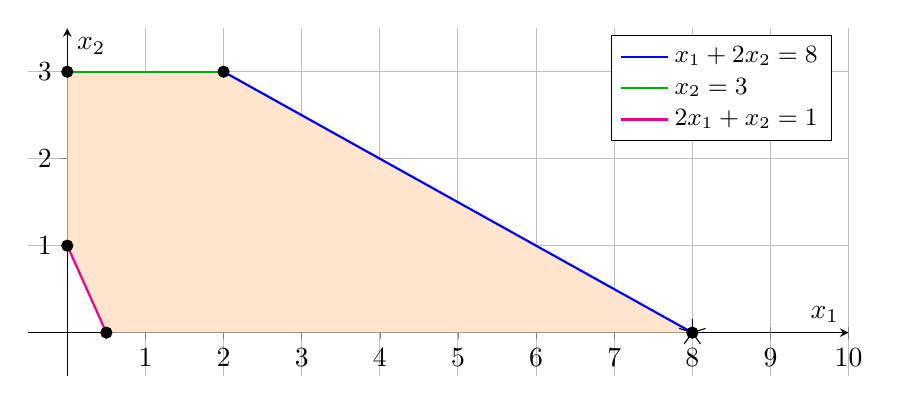
\begin{tikzpicture}
                \begin{axis}[
                    width=12cm,
                    height=6cm,
                    axis lines=middle,
                    xmin=-0.5,xmax=10,
                    ymin=-0.5,ymax=3.5,
                    xlabel={$x_1$},
                    ylabel={$x_2$},
                    grid=both,
                    legend cell align=left,
                    legend style={font=\small,at={(0.98,0.98)},anchor=north east},
                    clip=false]

                    \addplot[
                      draw=none,
                      fill=orange!20,
                      forget plot
                    ] coordinates{
                      (0.5,0)(8,0)(2,3)(0,3)(0,1)
                    } -- cycle;

                    \addplot[
                      domain=2:8,
                      samples=2,
                      thick,
                      color=blue
                    ]{(8-x)/2};
                    \addlegendentry{$x_{1}+2x_{2}=8$}

                    \addplot[
                      domain=0:2,
                      samples=2,
                      thick,
                      color=green!70!black
                    ]{3};
                    \addlegendentry{$x_{2}=3$}

                    \addplot[
                      domain=0:0.5,
                      samples=2,
                      thick,
                      color=magenta
                    ]{1-2*x};
                    \addlegendentry{$2x_{1}+x_{2}=1$}

                    \addplot[only marks,mark=*] coordinates{
                    (0.5,0) (8,0) (2,3) (0,3) (0,1)
                    };

                    \addplot[only marks,mark=star,mark size=5,fill=red] coordinates {(8,0)};

                \end{axis}
            \end{tikzpicture}
        \end{center}

        直线对应约束条件,橙色区域为可行域。可行基解为$(0.5,0),(8,0),(2,3),(0,3),(0,1)$,

        对应值为$1,16,13,9,3$,因此最优解为$(8,0)$,对应目标函数值为$16$,存在唯一最优解。
    \end{solution}

    \begin{homework}[6pts]
        将下列线性规划问题化为标准形式,并列出初始单纯形表.
        \begin{flalign*}
            \min \quad&z=-x_1+2x_2-3x_3+2x_4 \\
            \st \quad& 4x_1-x_2+2x_3-x_4=-2 \\
            &x_1+x_2-x_3+2x_4\leq 14 \\
            &-2x_1+3x_2+x_3-x_4\geq 2 \\
            & x_1,x_2,x_3\geq 0, x_4\,\text{无约束}
        \end{flalign*}
    \end{homework}

    \begin{solution}
        令$x_4=x_5-x_6,x_5,x_6\geq 0$,对后两个不等式约束添加松弛变量$x_7,x_8$,则标准形式为:
        \begin{flalign*}
            \max \quad&z=x_1-2x_2+3x_3-2x_5+2x_6 \\
            \st \quad& -4x_1+x_2-2x_3+x_5-x_6=2 \\
            &x_1+x_2-x_3+2x_5-2x_6+x_7=14 \\
            &-2x_1+3x_2+x_3-x_5+x_6-x_8=2 \\
            & x_1,x_2,x_3, x_5,x_6,x_7,x_8\geq 0
        \end{flalign*}

        容易得到一组初始基可行解为$(x_1,x_2,x_3,x_5,x_6,x_7,x_8)=(0,2,0,0,0,12,4)$,

        对应目标函数值为$-4$,初始单纯形表如下:

        \begin{table}[H]
            \centering
            \begin{tabular}{|c|c|c|c|c|c|c|c|c|c|}
                \hline
                \multicolumn{3}{|c|}{$c_j\rightarrow$} & $1$ & $-2$ & $3$ & $-2$ & $2$ & $0$ & $0$  \\
                \hline
                $c_B$ & $x_B$ & $b$ & $x_1$ & $x_2$ & $x_3$ & $x_5$ & $x_6$ & $x_7$ & $x_8$ \\
                \hline
                $-2 $& $x_2$ & $2$ & $-4$ & $1$ & $-2$ & $1$ & $-1$ & $0$ & $0$\\
                \hline
                $0$ & $x_7$ & $12$ & $1$ & $1$ & $-1$ & $2$ & $-2$ & $1$ & $0$\\
                \hline
                $0$ & $x_8$ & $4$ & $-2$ & $3$ & $1$ & $-1$ & $1$ & $0$ & $-1$\\
                \hline
                \multicolumn{3}{|c|}{$\sigma_j$} & $-7$ & $0$ & $-1$ & $0$ & $0$ & $0$ & $0$\\
                \hline
            \end{tabular}
        \end{table}
    \end{solution}

    \begin{homework}[6pts]
        求下列线性规划问题中满足约束条件的所有基解,并指出哪些是基可行解,并代入目标函数,确定哪一个是最优解。
        \begin{flalign*}
            \max \quad& z=2x_1-x_2+3x_3+2x_4 \\
            \st \quad& 2x_1+3x_2-x_3-4x_4 = 8 \\
            &x_1-2x_2+6x_3-7x_4 = -3 \\
            &x_1,x_2,x_3,x_4\geq 0
        \end{flalign*}
    \end{homework}

    \begin{solution}
        有$2$个等式约束和$4$个变量,因此需要令除基变量的$2$个变量为$0$,以下为结果:

        \begin{table}[H]
            \centering
            \begin{tabular}{|c|c|c|c|c|}
                \hline
                基变量 & 解向量 & 是否可行 & 目标函数值 \\
                \hline
                $x_1,x_2$ & $(1,2,0,0)$ & 是 & $0$ \\
                \hline
                $x_1,x_3$ & $(\tfrac{45}{13},0,-\tfrac{14}{13},0)$ & 否 & N/A \\
                \hline
                $x_1,x_4$ & $(\tfrac{34}5,0,0,\tfrac75)$ & 是 & $\tfrac{82}5$ \\
                \hline
                $x_2,x_3$ & $(0,\tfrac{45}{16},\tfrac7{16},0)$ & 是 & $-\tfrac32$ \\
                \hline
                $x_2,x_4$ & $(0,\tfrac{68}{29},0,-\tfrac7{29})$ & 否 & N/A \\
                \hline
                $x_2,x_3$ & $(0,0,-\tfrac{68}{31},-\tfrac{45}{31})$ & 否 & N/A \\
                \hline
            \end{tabular}
        \end{table}
    \end{solution}

    \begin{homework}[6pts]
        用单纯形方法求解以下线性规划问题:
        \begin{flalign*}
            \max \quad& z=3x_1-2x_2+5x_3 \\
            \st \quad &3x_1+2x_3\leq 13 \\
            & x_2+3x_3\leq 17 \\
            &2x_1+x_2+x_3\leq 13 \\
            &x_1,x_2,x_3\geq0
        \end{flalign*}
    \end{homework}

    \begin{solution}
        对约束条件添加松弛变量$x_4,x_5,x_6$,则标准形式为:
        \begin{flalign*}
            \max \quad& z=3x_1-2x_2+5x_3 \\
            \st \quad &3x_1+2x_3+x_4=13 \\
            & x_2+3x_3+x_5=17 \\
            &2x_1+x_2+x_3+x_6=13 \\
            &x_1,x_2,x_3,x_4,x_5,x_6\geq 0
        \end{flalign*}

        一组初始基可行解为$(x_1,x_2,x_3,x_4,x_5,x_6)=(0,0,0,13,17,13)$,初始单纯形表如下:

        \begin{table}[H]
            \centering
            \begin{tabular}{|c|c|c|c|c|c|c|c|c|}
                \hline
                \multicolumn{3}{|c|}{$c_j\rightarrow$} & $3$ & $-2$ & $5$ & $0$ & $0$ & $0$ \\
                \hline
                $c_B$ & $x_B$ & $b$ & $x_1$ & $x_2$ & $x_3$ & $x_4$ & $x_5$ & $x_6$ \\
                \hline
                $0$& $x_4$ & $13$ & $3$ & $0$ & $2$ & $1$ & $0$ & $0$\\
                \hline
                $0$& $x_5$ & $17$ & $0$ & $1$ & $3$ & $0$ & $1$ & $0$\\
                \hline
                $0$& $x_6$ & $13$ & $2$ & $1$ & $1$ & $0$ & $0$ & $1$\\
                \hline
                \multicolumn{3}{|c|}{$\sigma_j$} & $3$ & $-2$ & $5$ & $0$ & $0$ & $0$\\
                \hline
            \end{tabular}
        \end{table}

        以下进行单纯形表迭代:

        \begin{table}[H]
            \centering
            \begin{tabular}{|c|c|c|c|c|c|c|c|c|}
                \hline
                \multicolumn{3}{|c|}{$c_j\rightarrow$} & $3$ & $-2$ & $5$ & $0$ & $0$ & $0$ \\
                \hline
                $c_B$ & $x_B$ & $b$ & $x_1$ & $x_2$ & $x_3$ & $x_4$ & $x_5$ & $x_6$ \\
                \hline
                $0$& $x_4$ & $\tfrac{5}{3}$ & $3$ & $-\tfrac{2}{3}$ & $0$ & $1$ & $-\tfrac{2}{3}$ & $0$\\
                \hline
                $5$& $x_3$ & $\tfrac{17}{3}$ & $0$ & $\tfrac{1}{3}$ & $1$ & $0$ & $\tfrac{1}{3}$ & $0$\\
                \hline
                $0$& $x_6$ & $\tfrac{22}{3}$ & $2$ & $\tfrac{2}{3}$ & $0$ & $0$ & $-\tfrac{1}{3}$ & $1$\\
                \hline
                \multicolumn{3}{|c|}{$\sigma_j$} & $3$ & $-\tfrac{11}{3}$ & $0$ & $0$ & $-\tfrac{5}{3}$ & $0$\\
                \hline
            \end{tabular}
        \end{table}

        \begin{table}[H]
            \centering
            \begin{tabular}{|c|c|c|c|c|c|c|c|c|}
                \hline
                \multicolumn{3}{|c|}{$c_j\rightarrow$} & $3$ & $-2$ & $5$ & $0$ & $0$ & $0$ \\
                \hline
                $c_B$ & $x_B$ & $b$ & $x_1$ & $x_2$ & $x_3$ & $x_4$ & $x_5$ & $x_6$ \\
                \hline
                $3$& $x_1$ & $\tfrac59$ & $1$ & $-\tfrac29$ & $0$ & $\tfrac13$ & $-\tfrac29$ & $0$\\
                \hline
                $5$& $x_3$ & $\tfrac{17}3$ & $0$ & $\tfrac13$ & $1$ & $0$ & $\tfrac13$ & $0$\\
                \hline
                $0$& $x_6$ & $\tfrac{56}9$ & $0$ & $\tfrac{10}9$ & $0$ & $-\tfrac23$ & $\tfrac19$ & $1$\\
                \hline
                \multicolumn{3}{|c|}{$\sigma_j$} & $0$ & $-3$ & $0$ & $-1$ & $-1$ & $0$\\
                \hline
            \end{tabular}
        \end{table}

        因此最优解为$\left(\dfrac59,0,\dfrac{17}3,0,0,\dfrac{56}9\right)$,对应目标函数值为$30$。
    \end{solution}

    \begin{homework}[6pts]
        用大M法求解下列线性规划问题:
        \begin{flalign*}
            \min \quad& z=3x_1-x_2 \\
            \st \quad& 3x_1+x_2\geq 3 \\
            &2x_1-3x_2\geq 1\\
            &x_1,x_2\geq 0
        \end{flalign*}
    \end{homework}

    \begin{solution}
        对约束条件添加松弛变量$x_3,x_4$,并添加人工变量$x_5,x_6$,则标准形式为:
        \begin{flalign*}
            \max \quad& z=-3x_1+x_2-Mx_5-Mx_6 \\
            \st \quad& 3x_1+x_2-x_3+x_5=3 \\
            &2x_1-3x_2-x_4+x_6=1 \\
            & x_1,x_2,x_3,x_4,x_5,x_6\geq 0
        \end{flalign*}

        初始基可行解为$(x_1,x_2,x_3,x_4,x_5,x_6)=(0,0,0,0,3,1)$,初始单纯形表如下:

        \begin{table}[H]
            \centering
            \begin{tabular}{|c|c|c|c|c|c|c|c|c|}
                \hline
                \multicolumn{3}{|c|}{$c_j\rightarrow$} & $-3$ & $1$ & $0$ & $0$ & $-M$ & $0$ \\
                \hline
                $c_B$ & $x_B$ & $b$ & $x_1$ & $x_2$ & $x_3$ & $x_4$ & $x_5$ & $x_6$ \\
                \hline
                $-M$& $x_5$ & $3$ & $3$ & $1$ & $-1$ & $0$ & $1$ & $0$\\
                \hline
                $-M$& $x_6$ & $1$ & $2$ & $-3$ & $0$ & $-1$ & $0$ & $1$\\
                \hline
                \multicolumn{3}{|c|}{$\sigma_j$} & $5M-3$ & $1-2M$ & $-M$ & $-M$ & $0$ & $0$\\
                \hline
            \end{tabular}
        \end{table}

        以下进行单纯形表迭代:

        \begin{table}[H]
            \centering
            \begin{tabular}{|c|c|c|c|c|c|c|c|c|}
                \hline
                \multicolumn{3}{|c|}{$c_j\rightarrow$} & $-3$ & $1$ & $0$ & $0$ & $-M$ & $0$ \\
                \hline
                $c_B$ & $x_B$ & $b$ & $x_1$ & $x_2$ & $x_3$ & $x_4$ & $x_5$ & $x_6$ \\
                \hline
                $-M$& $x_5$ & $\tfrac32$ & $0$ & $\tfrac{11}2$ & $-1$ & $\tfrac32$ & $1$ & $-\tfrac32$\\
                \hline
                $-3$& $x_1$ & $\tfrac12$ & $1$ & $-\tfrac32$ & $0$ & $-\tfrac12$ & $0$ & $\tfrac12$\\
                \hline
                \multicolumn{3}{|c|}{$\sigma_j$} & $0$ & $\tfrac{11M-7}2$ & $-M$ & $\tfrac{3M}2$ & $0$ & $\tfrac{3-5M}2$\\
                \hline
            \end{tabular}
        \end{table}

        \begin{table}[H]
            \centering
            \begin{tabular}{|c|c|c|c|c|c|c|c|c|}
                \hline
                \multicolumn{3}{|c|}{$c_j\rightarrow$} & $-3$ & $1$ & $0$ & $0$ & $-M$ & $0$ \\
                \hline
                $c_B$ & $x_B$ & $b$ & $x_1$ & $x_2$ & $x_3$ & $x_4$ & $x_5$ & $x_6$ \\
                \hline
                $1$& $x_2$ & $\tfrac3{11}$ & $0$ & $1$ & $-\tfrac2{11}$ & $\tfrac3{11}$ & $\tfrac2{11}$ & $-\tfrac3{11}$\\
                \hline
                $-3$& $x_1$ & $\tfrac{10}{11}$ & $1$ & $0$ & $-\tfrac3{11}$ & $-\tfrac1{11}$ & $\tfrac3{11}$ & $\tfrac1{11}$\\
                \hline
                \multicolumn{3}{|c|}{$\sigma_j$} & $0$ & $0$ & $-\tfrac7{11}$ & $-\tfrac6{11}$ & $\tfrac7{11}-M$ & $\tfrac6{11}-M$ \\
                \hline
            \end{tabular}
        \end{table}

        因此最优解为$\left(\dfrac{10}{11},\dfrac{3}{11},0,0,0,0\right)$,对应目标函数值为$-\dfrac{27}{11}$。
    \end{solution}

    \begin{homework}[6pts]
        分别用最速下降法与牛顿法求函数$f(x)=x_1^2-x_1 x_2
        +x_2^2+x_1 x_3+x_3^2-2x_1+4x_2+2x_3-2, x=(x_1,x_2,x_3)^{\top}\in\mathbb{R}^3$的极小点, 初始点$x_0=(0,0,0)^{\top}$,要求:
        \begin{enumerate}
            \item 最速下降法进行$2$次迭代, 并验证相邻两步的搜索方向正交;
            \item 牛顿法进行1次迭代。
        \end{enumerate}
    \end{homework}

    \begin{solution}
        $\nabla f=(2x_1-x_2+x_3-2,-x_1+2x_2+4,x_1+2x_3+2)^{\top},\nabla^2 f=\begin{bmatrix}2&-1&1\\-1&2&0\\1&0&2\end{bmatrix}$。

        对于最速下降法,初始点为$x_0=(0,0,0)^{\top},d_0=\nabla f(x_0)=(-2,4,2)^{\top}$,

        $\alpha_0=\argmin_{\alpha}f(x_0+\alpha d_0)=\argmin_{\alpha}(28\alpha^2-24\alpha-2)=\dfrac37$,

        $x_1=x_0+\alpha_0 d_0=\left(\dfrac67,-\dfrac{12}7,-\dfrac67\right)^{\top},d_1=\nabla f(x_1)=\left(\dfrac47,-\dfrac27,\dfrac87\right)^{\top},\langle d_0,d_1\rangle=0$,

        $\alpha_1=-\dfrac{\nabla f(x_1)^{\top}d_1}{d_1^{\top}\nabla^2 f(x_1)d_1}=\dfrac{21}{62},x_2=x_1+\alpha_1 d_1=\left(\dfrac{144}{217},-\dfrac{351}{217},-\dfrac{270}{217}\right)^{\top}$,

        对于牛顿法,$x_1=x_0-\nabla^2 f(x_0)^{-1}\nabla f(x_0)=\left(1,-\dfrac32,\dfrac32\right)^{\top}$,

        由于$\nabla^2 f\succ 0,\nabla f(x)=0$时$x^*=\left(1,-\dfrac32,\dfrac32\right)^{\top}$,有$x^*$为全局最优解,$f(x^*)=-\dfrac{15}2$。
    \end{solution}

\end{document}


